\section{Data Description}\label{sec:data_description}
The primary data this paper employs are located menu expenditures, which contain the yearly allotted allocations from aldermen and their respective locations from 2005 to 2022.
This dataset comes from menu spending reports that are publicly available from 2011 through 2022, and records that were not previously publicly available that were obtained through a FOIA request to the OBM \cite{OBM_datasource}.  
I then scraped these PDFs and used the resulting cost total, ward, and location description data to create a map of shapes of the locations of the expenditures.
I then used the location description text to locate each project's described vertices using the Census geocoding API. 
If the Census's API failed, I automatically used Google Maps' API instead.
In total, 43,596 projects needed to be located, and 83\% of them were successfully located using one of the above methods.
For example, spending on playground equipment would be a singular point, while spending on a street would be a line, and spending on all alleys within a given block would be a polygon.
The spending for each project was then allocated to the precincts that it overlapped with, by area.
If there was a \$10,000 quadrangle of $500 m^2$ and 60\% of it was in precinct A and 40\% was in precinct B, then 60\% of the spending on that project would be allocated to precinct A and 40\% to precinct B.
Lines, such as street resurfacing, were allocated by length.
This dataset contains 41,381 precinct-year observations, which record the total spending in a given voting precinct in a given year.

Figure~\ref{fig:spending_hist} depicts two side-by-side histograms of the distribution of spending per precinct aggregated across the 2005-2011 period, which used the 2003-2011 ward boundaries and the 2012-2022 period with the 2012-2022 ward boundaries.
The decentralized nature of the menu program leads to a considerable variation in spending per precinct, but the distribution has a long right tail.
Both figures are winsorized at the 99th percentile to remove outliers.

\begin{figure}[H]
    \centering
    % First subfigure
    \begin{subfigure}[b]{0.45\textwidth} % [b] aligns at the bottom
      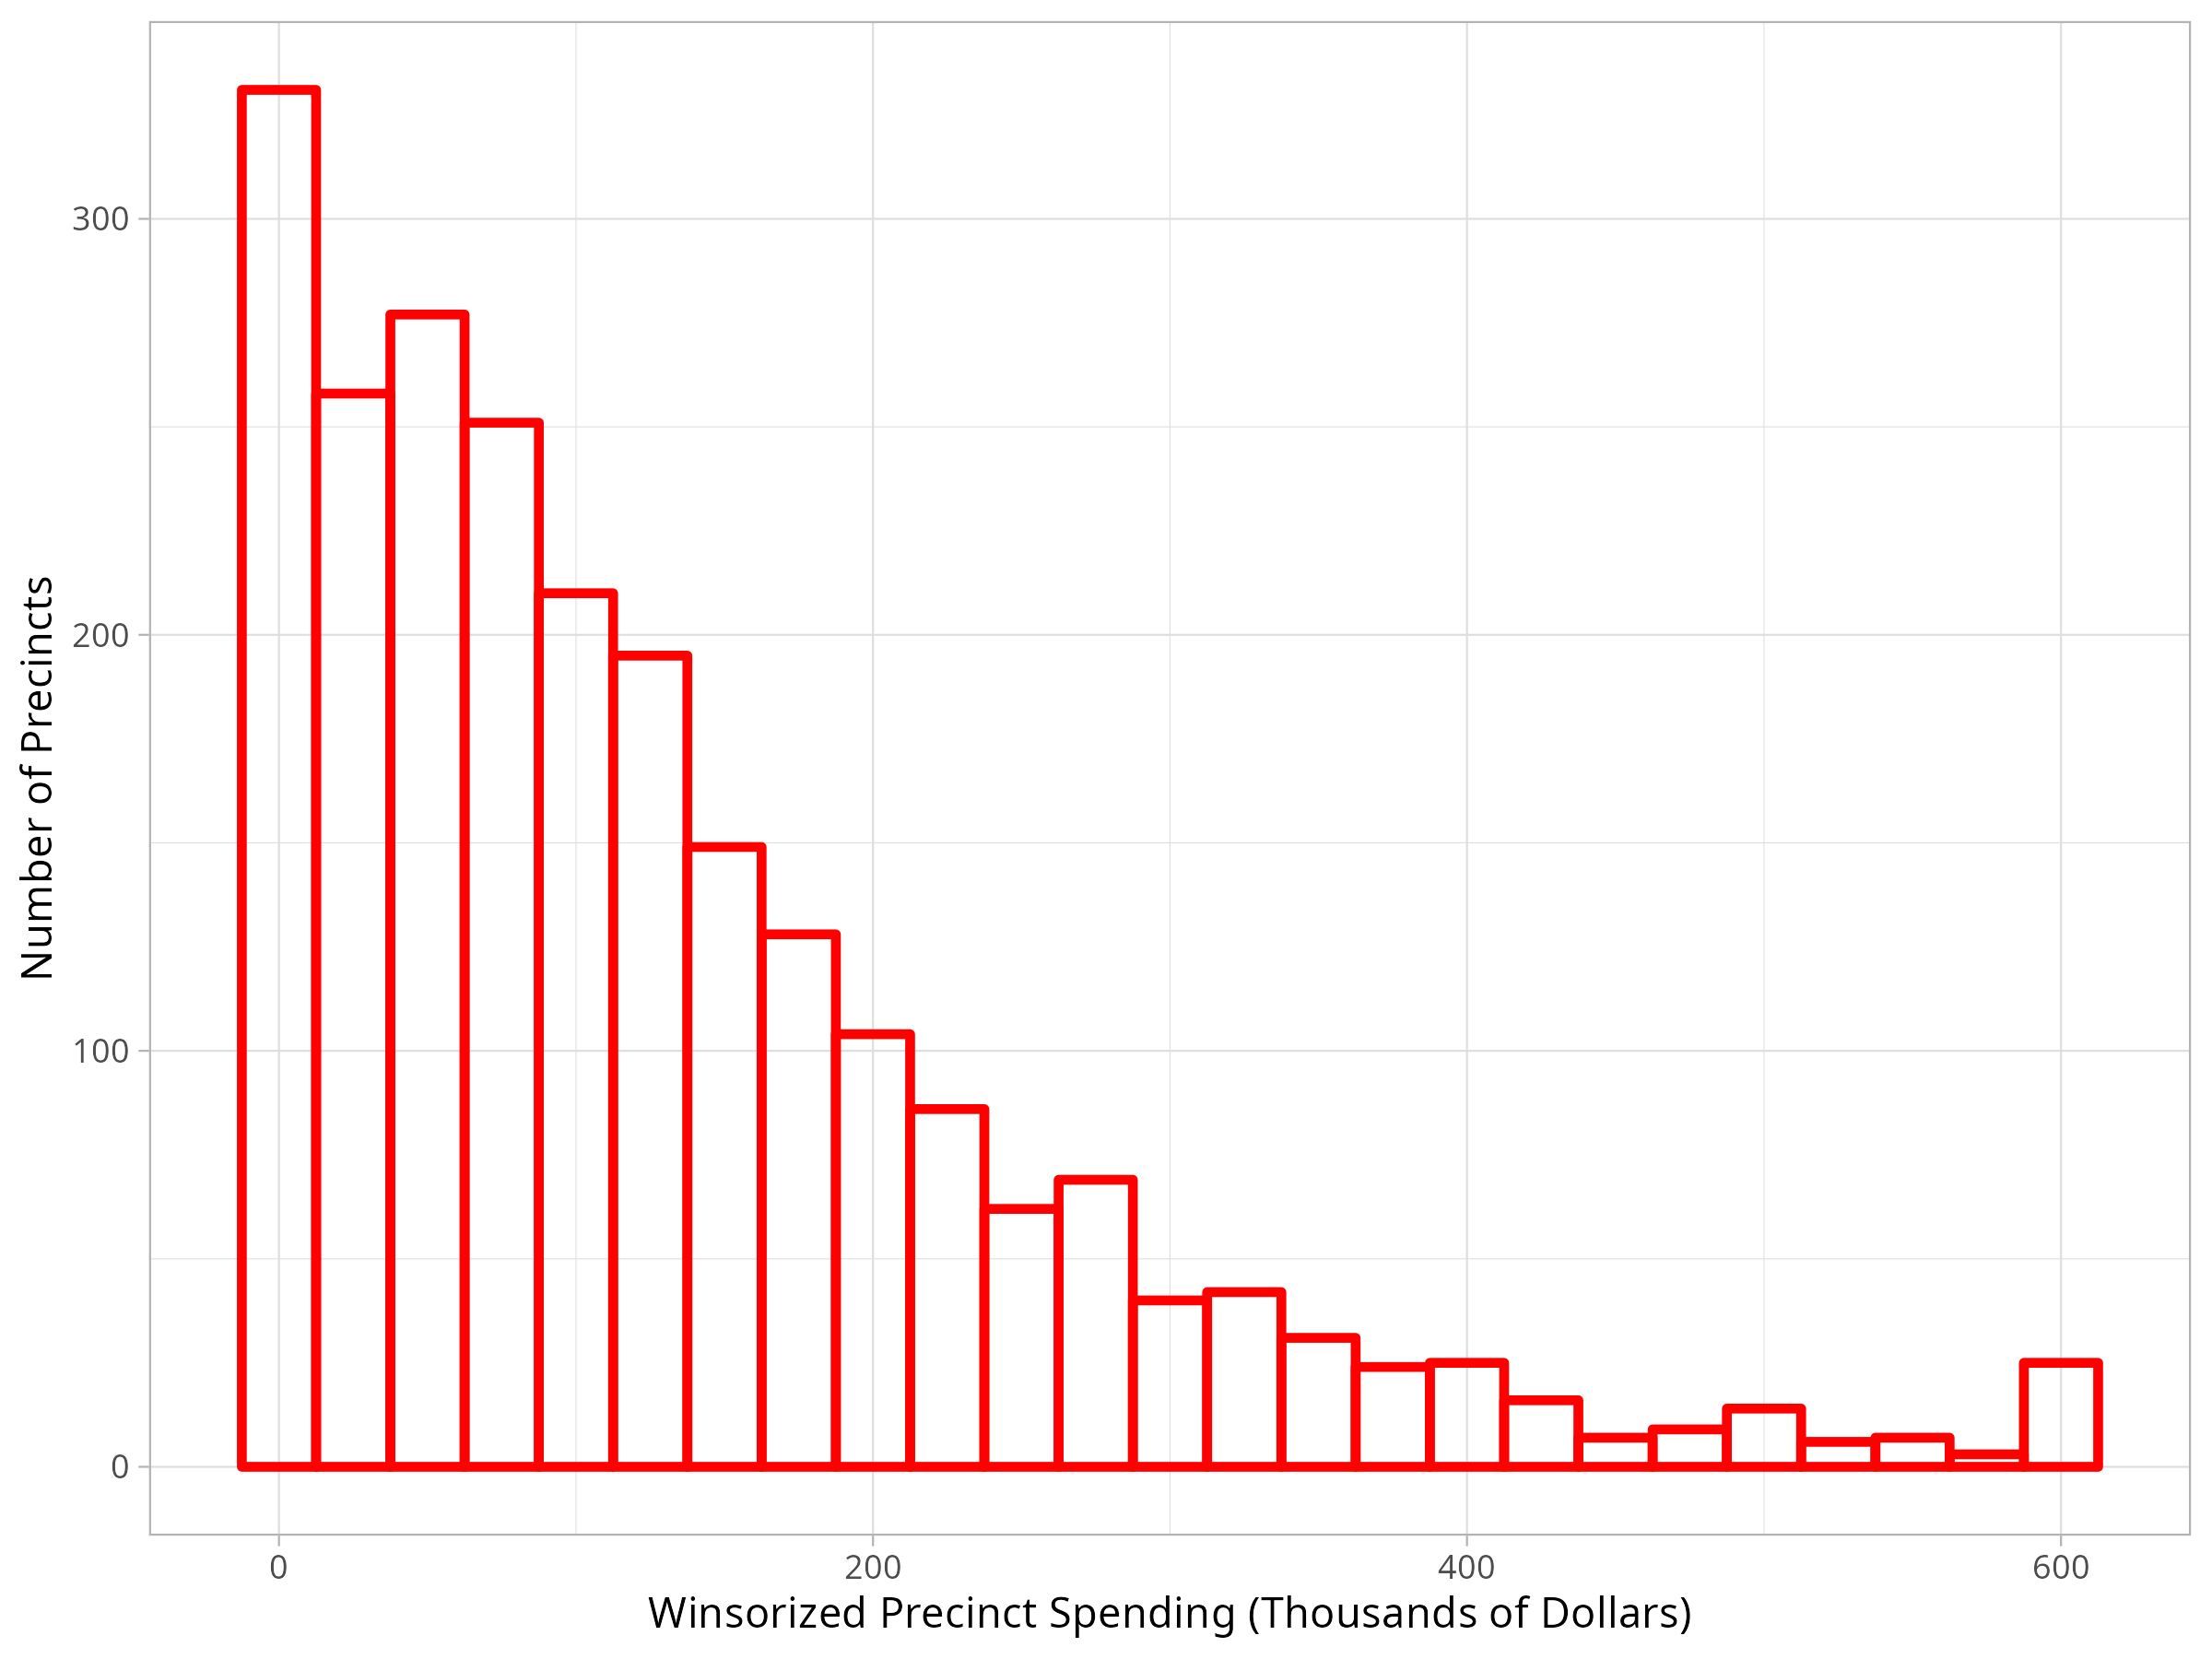
\includegraphics[width=\textwidth]{input/spending_histogram_2005_2011.png}
      \caption{2005-2011}
      \label{fig:sub1}
    \end{subfigure}
    \hfill % This adds some space between the two subfigures
    % Second subfigure
    \begin{subfigure}[b]{0.45\textwidth}
      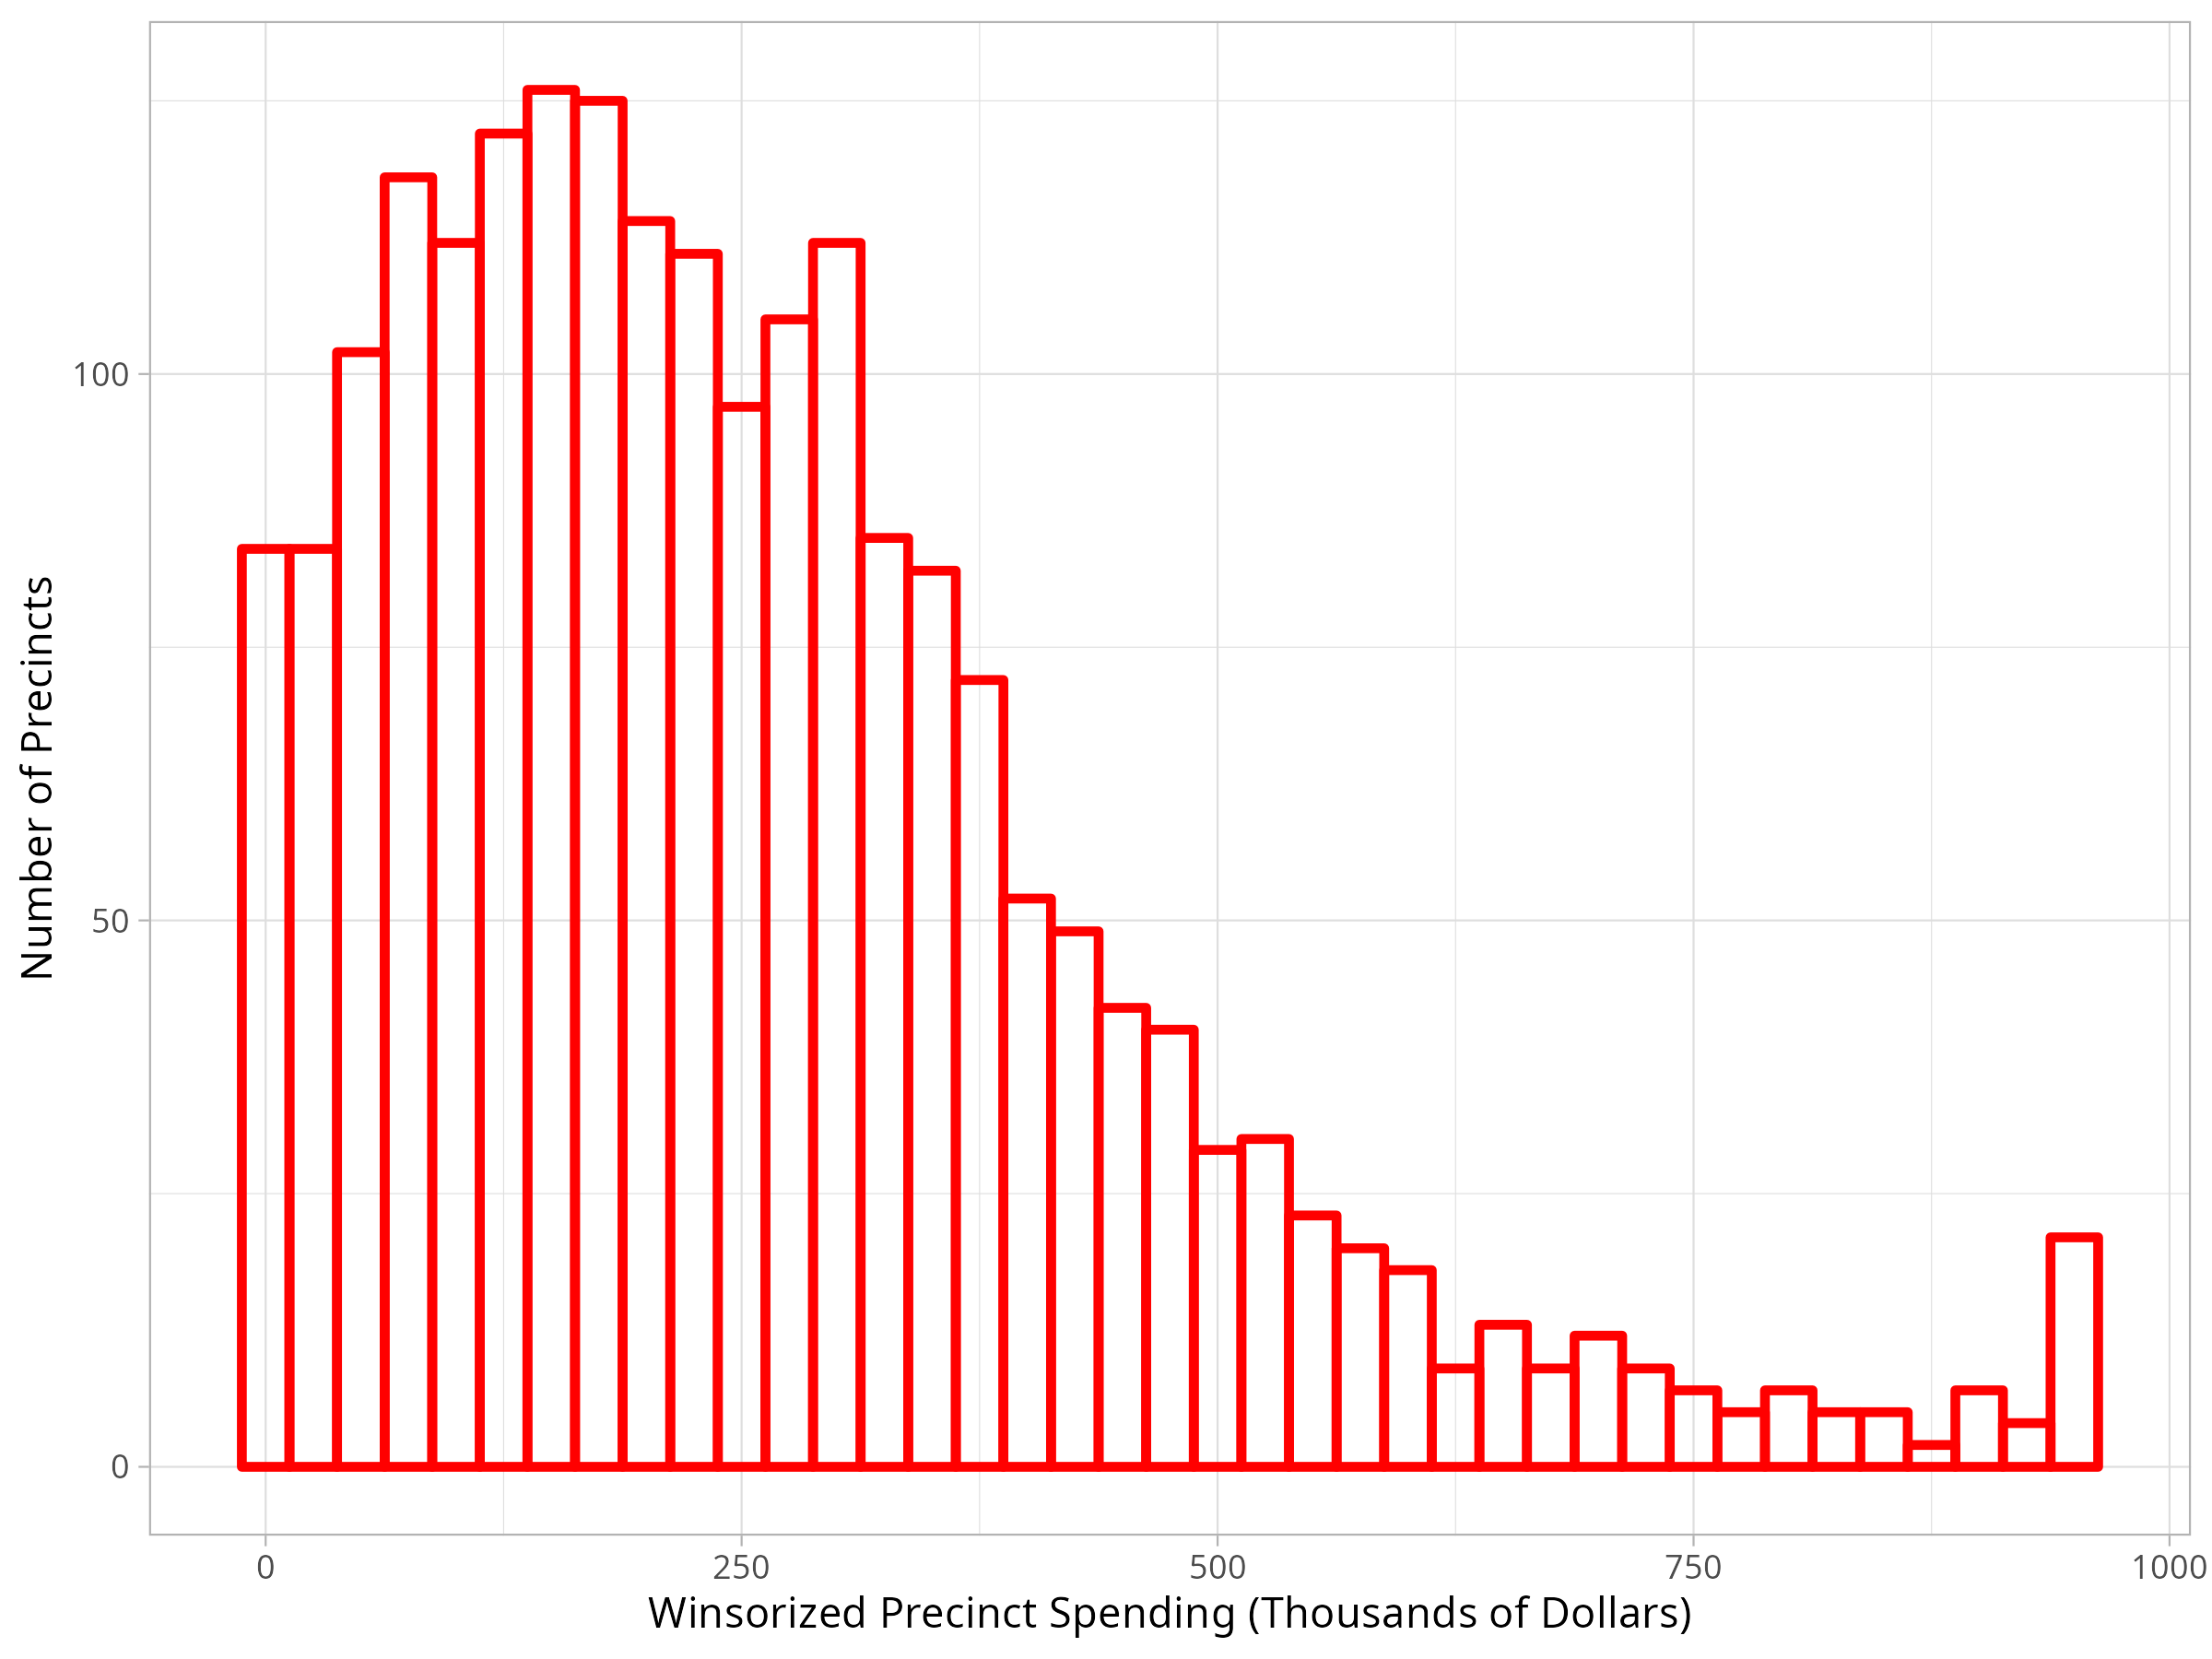
\includegraphics[width=\textwidth]{input/spending_histogram_2012_2022.png}
      \caption{2012-2022}
      \label{fig:sub2}
    \end{subfigure}
  
    \caption{Distribution of Spending per Precinct for both ward maps in the dataset}
    \label{fig:spending_hist}
  \end{figure}

Next, Figure~\ref{fig:spending_map} depicts within-ward spending variation across Chicago using the 2012-2022 precinct map; spending is often concentrated in a few precincts.

\begin{figure}[H]
    \centering
    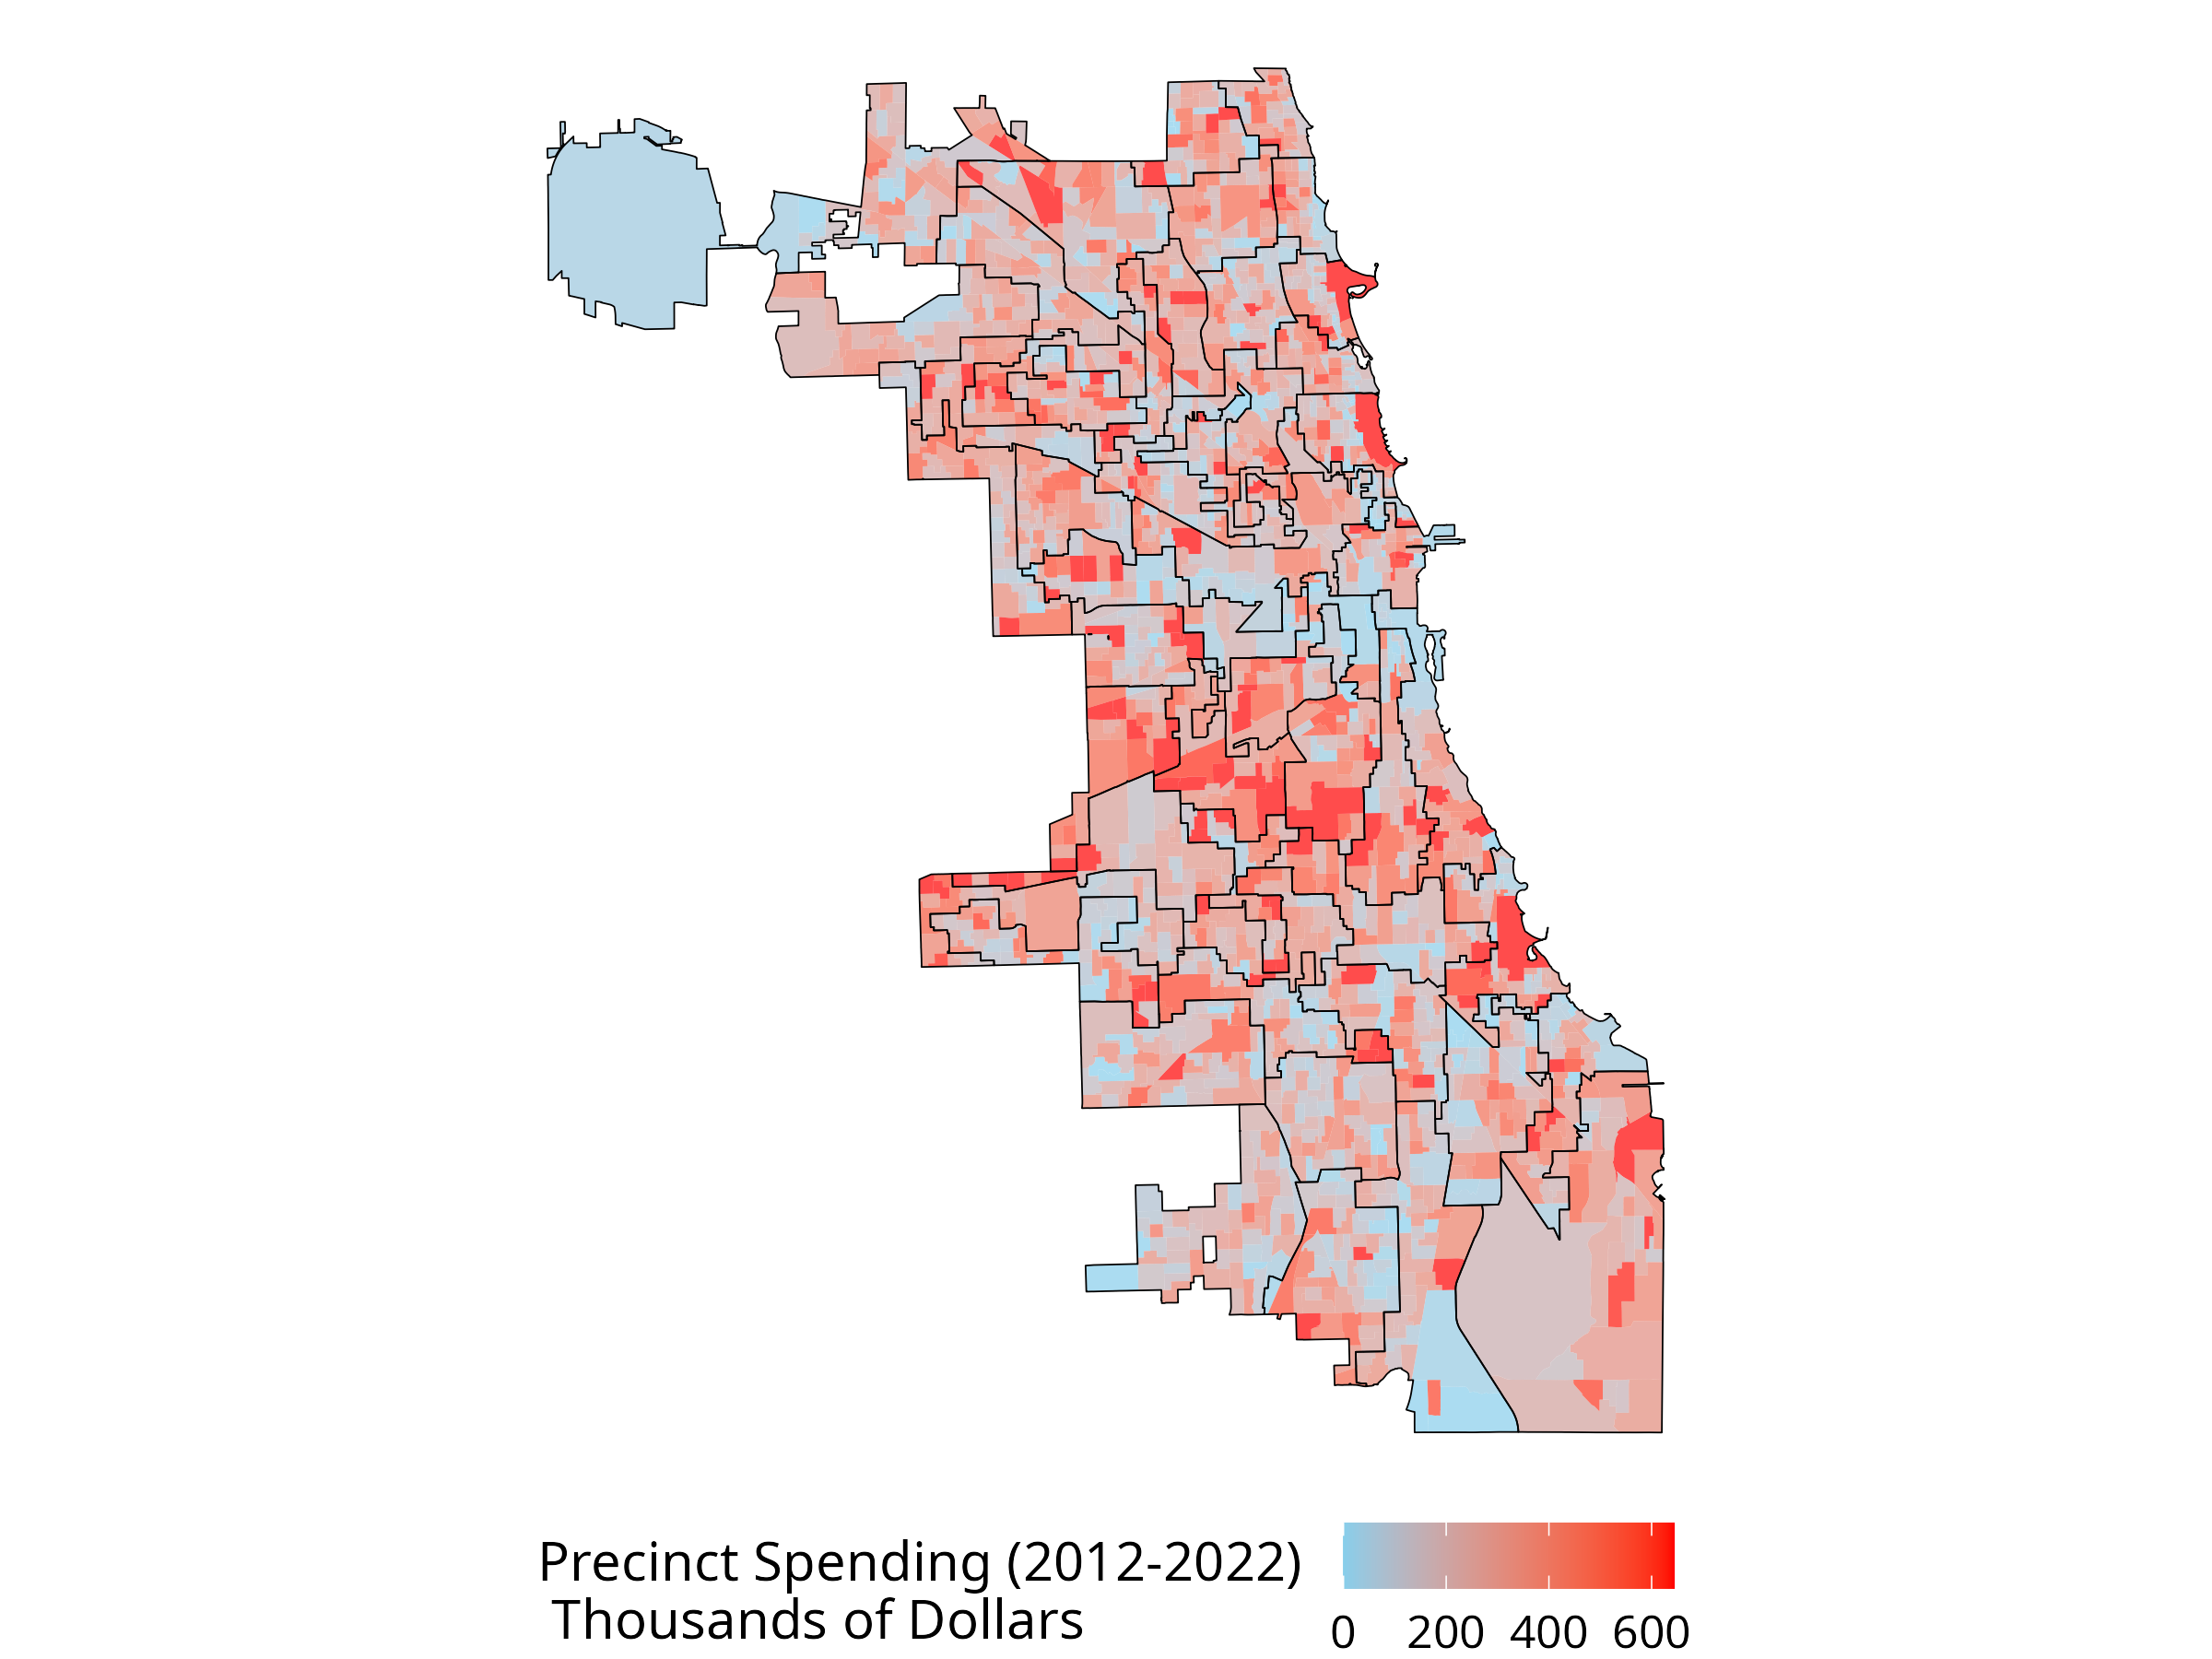
\includegraphics[width=0.65\textwidth]{input/whole_chicago_map_2012_2022.png}
    \caption{Map of Spending per Precinct, 2012-2022}
    \label{fig:spending_map}
\end{figure}

To avoid issues with different levels of ``observable'' spending from year to year, I use the fraction of spending located in a precinct in a given year as the dependent variable for subsequent analyses.
For example, if a precinct received \$50,000 in spending in 2019, but only \$900,000 of its wards \$1,5M budget was located, then the fraction of spending located in that precinct in 2019 of its ward's 2019 spending would be $\frac{50,000}{900,000}*100 =5.6\%$.
This is important because the amount of observable spending can shift from year to year, but that doesn't mean that alderman is prioritizing the precinct any less that year, necessarily.
``Observed'' means one of the two methods above successfully located it to a location in Chicago.
Thus, if $Y_{py}$ is the fraction of spending located in precinct $p$ in year $y$, then $Y_{py} = \frac{S_{py}}{S_{wy}}$, where $S_{py}$ is the spending in precinct $p$ in year $y$, and $S_{wy}$ is the total amount of ward $w$'s successfully located spending in year $y$.
Table~\ref{summary_stats} depicts summary statistics for this variable.
Due to the long right tail of the distribution, the mean is much larger than the median.
Half of precincts get almost no spending.

\begin{table}[H]
\caption{Summary statistics of fraction of total spending by precinct from 2012 to 2022}\label{summary_stats}
\centering
\begin{tabular}[t]{ccccc}
\toprule
mean & median & sd & upper quartile & lower quartile\\
\midrule
2.42 & 0.23 & 4.48 & 3.35 & 0\\
\bottomrule
\end{tabular}
\end{table}